\documentclass[hidelinks,12pt]{article}
\usepackage[left=0.25cm,top=1cm,right=0.25cm,bottom=1cm]{geometry}
%\usepackage[landscape]{geometry}
\textwidth = 20cm
\hoffset = -1cm
\usepackage[utf8]{inputenc}
\usepackage[spanish,es-tabla]{babel}
\usepackage[autostyle,spanish=mexican]{csquotes}
\usepackage[tbtags]{amsmath}
\usepackage{nccmath}
\usepackage{amsthm}
\usepackage{amssymb}
\usepackage{mathrsfs}
\usepackage{graphicx}
\usepackage{subfig}
\usepackage{standalone}
\usepackage[outdir=./Imagenes/]{epstopdf}
\usepackage{siunitx}
\usepackage{physics}
\usepackage{color}
\usepackage{float}
\usepackage{hyperref}
\usepackage{multicol}
%\usepackage{milista}
\usepackage{anyfontsize}
\usepackage{anysize}
%\usepackage{enumerate}
\usepackage[shortlabels]{enumitem}
\usepackage{capt-of}
\usepackage{bm}
\usepackage{relsize}
\usepackage{placeins}
\usepackage{empheq}
\usepackage{cancel}
\usepackage{wrapfig}
\usepackage[flushleft]{threeparttable}
\usepackage{makecell}
\usepackage{fancyhdr}
\usepackage{tikz}
\usepackage{bigints}
\usepackage{scalerel}
\usepackage{pgfplots}
\usepackage{pdflscape}
\pgfplotsset{compat=1.16}
\spanishdecimal{.}
\renewcommand{\baselinestretch}{1.5} 
\renewcommand\labelenumii{\theenumi.{\arabic{enumii}})}
\newcommand{\ptilde}[1]{\ensuremath{{#1}^{\prime}}}
\newcommand{\stilde}[1]{\ensuremath{{#1}^{\prime \prime}}}
\newcommand{\ttilde}[1]{\ensuremath{{#1}^{\prime \prime \prime}}}
\newcommand{\ntilde}[2]{\ensuremath{{#1}^{(#2)}}}

\newtheorem{defi}{{\it Definición}}[section]
\newtheorem{teo}{{\it Teorema}}[section]
\newtheorem{ejemplo}{{\it Ejemplo}}[section]
\newtheorem{propiedad}{{\it Propiedad}}[section]
\newtheorem{lema}{{\it Lema}}[section]
\newtheorem{cor}{Corolario}
\newtheorem{ejer}{Ejercicio}[section]

\newlist{milista}{enumerate}{2}
\setlist[milista,1]{label=\arabic*)}
\setlist[milista,2]{label=\arabic{milistai}.\arabic*)}
\newlength{\depthofsumsign}
\setlength{\depthofsumsign}{\depthof{$\sum$}}
\newcommand{\nsum}[1][1.4]{% only for \displaystyle
    \mathop{%
        \raisebox
            {-#1\depthofsumsign+1\depthofsumsign}
            {\scalebox
                {#1}
                {$\displaystyle\sum$}%
            }
    }
}
\def\scaleint#1{\vcenter{\hbox{\scaleto[3ex]{\displaystyle\int}{#1}}}}
\def\bs{\mkern-12mu}


\title{\large{Asesoría Repaso Tema 1} \vspace{-3ex}}
\author{M. en C. Gustavo Contreras Mayén}
\date{ }
\newcommand{\Cancel}[2][black]{{\color{#1}\cancel{\color{black}#2}}}
\begin{document}
\vspace{-4cm}
\maketitle
\fontsize{14}{14}\selectfont
\tableofcontents
\newpage

\section{Sistema de coordenadas generalizadas}
%Moon (1988) - Field Theory. Table 1.09 Conical coordinates
\subsection{Ejercicio de transformación}

Un sistema de coordenadas cónico que utiliza las coordenadas $(r, \theta, \lambda)$:
\begin{align*}
u^{1} &= r \hspace{1.5cm} 0 \leq r < \infty \\[0.5cm]
u^{2} &= \theta \hspace{1.5cm} 0 < \theta^{2} < c^{2} \\[0.5cm]
u^{3} &= \lambda \hspace{1.5cm} 0 < \lambda^{2} < b^{2} \\[0.5cm]
\end{align*}
Se puede formar a partir de las coordenadas cartesianas:
\begin{align*}
(x)^{2} &= \left( \dfrac{r \, \theta \, \lambda}{b \, c} \right)^{2} \\[0.5em]
(y)^{2} &= \dfrac{r^{2} \, (\theta^{2} - b^{2})(b^{2} - \lambda^{2})}{b^{2} \, (c^{2} - b^{2})} \\[0.5em]
(z)^{2} &= \dfrac{r^{2} \, (c^{2} - \theta^{2})(c^{2} - \lambda^{2})}{c^{2} \, (c^{2} - b^{2})}
\end{align*}
con $c^{2} > \theta^{2} > b^{2} > \lambda^{2} > 0$.

\textbf{Resuelve:}

\begin{enumerate}
\item Describe las superficies coordenadas para $r$, $\theta$ y $\lambda$ constantes.
\item Obtén los factores de escala $h_{i}$ para este sistema de coordenadas cónico.
\item Escribe las expresiones para los operadores diferenciales: gradiente $\grad \phi$, divergencia $\div{\vb{A}}$ y rotacional $\curl{\vb{A}}$.
\item ¿Cómo escribiríamos la ecuación de Laplace en este sistema de coordenadas cónico?
\end{enumerate}

\section{Solución del ejercicio}
\subsection{Superficies coordenadas}



Las superficies coordenadas son aquellas que se obtienen fijando sucesivamente cada una de las coordenadas de un punto.
Iniciamos con $r$ constante.
\par
Simplificamos el álgebra al expandir las expresiones para $y^{2}$ y $z^{2}$, para luego sumarlas:

\begin{align*}
y^{2} &= \dfrac{r^{2} \, \theta^{2}}{c^{2} - b^{2}} - \dfrac{r^{2} \, \theta^{2} \, \lambda^{2}}{b^{2}(c^{2} - b^{2})} - \dfrac{r^{2} \, b^{2}}{c^{2} - b^{2}} + \dfrac{r^{2} \, \lambda^{2}}{c^{2} - b^{2}} \\[1em] 
z^{2} &= \dfrac{r^{2} \, c^{2}}{c^{2} - b^{2}} - \dfrac{r^{2} \, \lambda^{2}}{c^{2} - b^{2}} - \dfrac{r^{2} \, \theta^{2}}{c^{2} - b^{2}} + \dfrac{r^{2} \, \theta^{2} \, \lambda^{2}}{c^{2} (c^{2} - b^{2})}
\end{align*}
\\
Tenemos entonces que:
\begin{align*}
y^{2} + z^{2} &= \Cancel[red]{\dfrac{r^{2} \, \theta^{2}}{c^{2} - b^{2}}} - \dfrac{r^{2} \, \theta^{2} \, \lambda^{2}}{b^{2}(c^{2} - b^{2})} - \dfrac{r^{2} \, b^{2}}{c^{2} - b^{2}} + \\[1em]
+& \Cancel[blue]{\dfrac{r^{2} \, \lambda^{2}}{c^{2} - b^{2}}} + \dfrac{r^{2} \, c^{2}}{c^{2} - b^{2}} - \Cancel[blue]{\dfrac{r^{2} \, \lambda^{2}}{c^{2} - b^{2}}} - \Cancel[red]{\dfrac{r^{2} \, \theta^{2}}{c^{2} - b^{2}}} + \\[0.5em]
&+ \dfrac{r^{2} \, \theta^{2} \, \lambda^{2}}{c^{2} (c^{2} - b^{2})} =
\end{align*}
\\
Al simplificar la expresión llegamos a:
\begin{align*}
y^{2} + z^{2} &= - \dfrac{r^{2} \, \theta^{2} \, \lambda^{2}}{b^{2}(c^{2} - b^{2})} - \dfrac{r^{2} \, b^{2}}{c^{2} - b^{2}} + \\[1em]
&+ \dfrac{r^{2} \, c^{2}}{c^{2} - b^{2}} + \dfrac{r^{2} \, \theta^{2} \, \lambda^{2}}{c^{2} (c^{2} - b^{2})} =
\end{align*}
\\
Obtenemos el m.c.m. del denominador para resolver esta suma de fracciones.
\begin{align*}
&= \dfrac{-b^{2} c^{2} (r^{2} b^{2}) + b^{2} c^{2} (r^{2} c^{2}) - r^{2} c^{2} \theta^{2} \lambda^{2} + r^{2} b^{2} \theta^{2} \lambda^{2}}{b^{2} c^{2} (c^{2} - b^{2})} = \\[1em] 
&= \dfrac{-r^{2} c^{2} b^{4} + r^{2} b^{2} c^{4} - r^{2} \theta^{2} \lambda^{2} (c^{2} - b^{2})}{b^{2} c^{2} (c^{2} - b^{2})} = \\[1em] 
&= - \dfrac{r^{2} b^{2}}{c^{2} - b^{2}} + \dfrac{r^{2} c^{2}}{c^{2} - b^{2}} - \dfrac{r^{2} \theta^{2} \lambda^{2}}{b^{2} c^{2}} =
\end{align*}
\\
Seguimos simplificando la expresión:
\begin{align*}
y^{2} + z^{2} &= r^{2} \cancelto{1}{\left[ \dfrac{c^{2} + b^{2}}{c^{2} + b^{2}} \right]} - \dfrac{r^{2} \theta^{2} \lambda^{2}}{b^{2} c^{2}} = \\[1em]
&= r^{2} \left[ 1 - \dfrac{\theta^{2} \, \lambda^{2}}{b^{2} \, c^{2}} \right]
\end{align*}
\\
Ahora sumamos el término de $x^{2}$:
\begin{align*}
x^{2} + y^{2} + z^{2} &= \dfrac{r^{2} \, \theta^{2} \, \lambda^{2}}{b^{2} \, c^{2}} + r^{2} \left[ 1 - \dfrac{\theta^{2} \, \lambda^{2}}{b^{2} \, c^{2}} \right] = \\[1em] 
&= r^{2} \left[ 1 - \dfrac{\theta^{2} \, \lambda^{2}}{b^{2} \, c^{2}} + \dfrac{\theta^{2} \, \lambda^{2}}{b^{2} \, c^{2}} \right] = \\[1em] 
&= r^{2}
\end{align*}
\\
Que nos define una familia de esferas de radio $r =$ cte.
\par
Siguiendo el mismo procedimiento\footnote{Que recomendamos con buen ejercicio moral que realicen el desarrollo y corroboren el resultado obtenido.}, se determinan las superficies coordenadas para $\theta=$ constante y para $\lambda=$ constante:

Conos elípticos, con $\theta=$ cte.
\begin{align*}
\dfrac{x^{2}}{\theta^{2}} + \dfrac{y^{2}}{\theta^{2} - b^{2}} - \dfrac{z^{2}}{c^{2} - \theta^{2}} = 0
\end{align*}

Conos elípticos, con $\lambda=$ cte.
\begin{align*}
\dfrac{x^{2}}{\lambda^{2}} - \dfrac{y^{2}}{b^{2} - \lambda^{2}} - \dfrac{z^{2}}{c^{2} - \lambda^{2}} = 0
\end{align*}
Como podremos ver en la siguiente figura:
\begin{figure}[H]
   \centering
   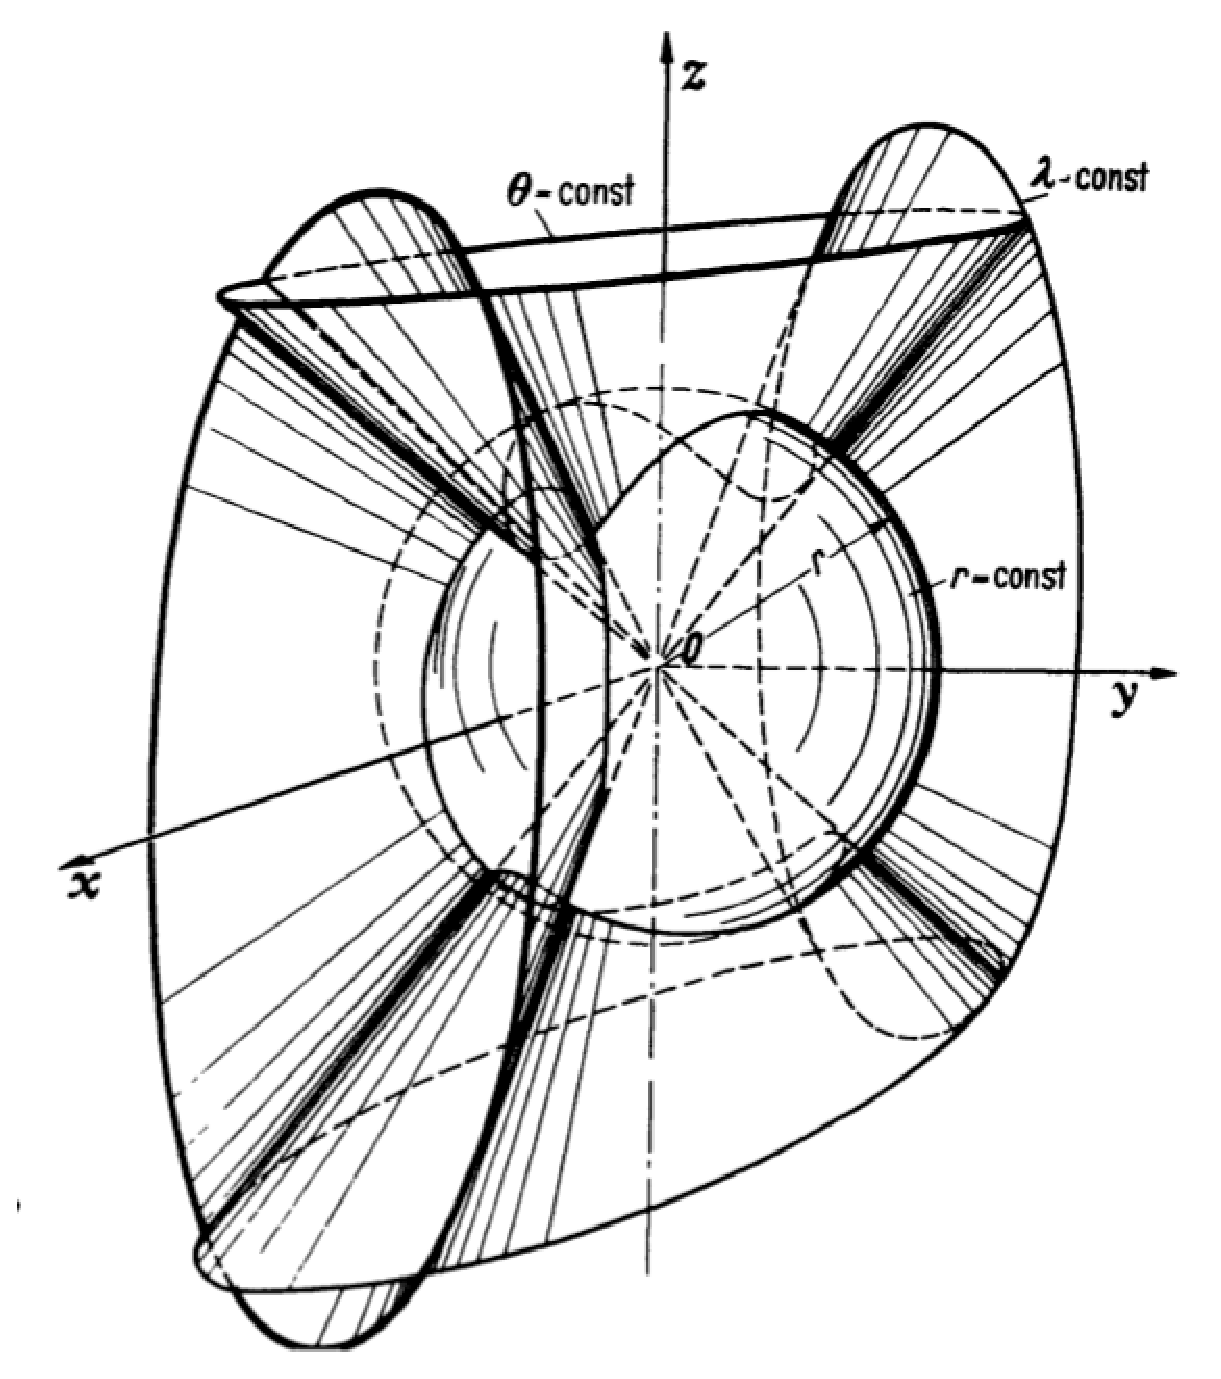
\includegraphics[scale=0.5]{Imagenes/Sistema_Conico.eps}
\end{figure}

\subsection{Factores de escala}

Calculamos los factores de escala o coeficientes métricos a partir de la expresión:
\begin{align*}
h_{i} &= \abs{\pdv{\vb{r}}{u_{i}}} \\[0.5em]
h_{i} &= \sqrt{ \left( \pdv{x}{u_{i}} \right)^{2} + \left( \pdv{y}{u_{i}} \right)^{2} + \left( \pdv{z}{u_{i}} \right)^{2}}
\end{align*}

Entonces el factor de escala  $h_{r}$ es:
\begin{align*}
h_{r} = \sqrt{\left( \pdv{x}{r} \right)^{2} + \left( \pdv{y}{r} \right)^{2} + \left( \pdv{z}{r} \right)^{2}}
\end{align*}

Con la finalidad de llevar la secuencia, calculemos primero las derivadas parciales con respecto a $r$, para luego elevarlas al cuadrado, luego las sumamos y obtenemos la raíz cuadrada.

\begin{align*}
x &= \dfrac{r \, \theta \, \lambda}{b \, c} \hspace{0.3cm} \Rightarrow \hspace{0.3cm}  \displaystyle \pdv{x}{r} = \dfrac{\theta \, \lambda}{b \, c} \\[1em] 
&\Rightarrow \displaystyle \left( \pdv{x}{r} \right)^{2} = \dfrac{\theta^{2} \, \lambda^{2}}{b^{2} \, c^{2}}
\end{align*}
\\
La derivada parcial de $y$ con respecto a $r$ es:
\begin{align*}
y &= \dfrac{r}{b} \sqrt{\dfrac{(\theta^{2} - b^{2})(b^{2} - \lambda^{2})}{(c^{2} - b^{2})}} \\[1em] 
&\Rightarrow \hspace{0.3cm} \displaystyle \pdv{y}{r} = \dfrac{1}{b} \sqrt{\dfrac{(\theta^{2} - b^{2})(b^{2} - \lambda^{2})}{(c^{2} - b^{2})}} \\[1em] 
&\Rightarrow \left( \pdv{y}{r} \right)^{2} = \dfrac{1}{b^{2}} \left( \dfrac{(\theta^{2} - b^{2})(b^{2} - \lambda^{2})}{(c^{2} - b^{2})}\right)
\end{align*}
\\
Mientras que la derivada parcial de $z$ con respecto a $r$ es:
\begin{align*}
z &= \dfrac{r}{c} \sqrt{\dfrac{(c^{2} - \theta^{2})(c^{2} - \lambda^{2})}{(c^{2} - b^{2})}} \\[1em] 
&\Rightarrow \hspace{0.3cm} \displaystyle \pdv{z}{r} = \dfrac{1}{c} \sqrt{\dfrac{(c^{2} - \theta^{2})(c^{2} - \lambda^{2})}{(c^{2} - b^{2})}} \\[1em] 
&\Rightarrow \left( \pdv{z}{r} \right)^{2} = \dfrac{1}{c^{2}} \left( \dfrac{(c^{2} - \theta^{2})(c^{2} - \lambda^{2})}{(c^{2} - b^{2})} \right)
\end{align*}
\\
Ahora podemos hacer la suma del cuadrado de las parciales:
\begin{align*}
&{} \left( \pdv{x}{r} \right)^{2} + \left( \pdv{y}{r} \right)^{2} + \left( \pdv{z}{r} \right)^{2} = \\[0.5em] 
&= \dfrac{\theta^{2} \, \lambda^{2}}{b^{2} \, c^{2}} + \dfrac{(\theta^{2} - b^{2})(b^{2} - \lambda^{2})}{b^{2} (c^{2} - b^{2})} + \dfrac{(c^{2} - \theta^{2})(c^{2} - \lambda^{2})}{c^{2} (c^{2} - b^{2})}
\end{align*}
\\
Desarrollamos la expresión y veamos qué términos se pueden cancelar:
\begin{align*}
&= \dfrac{\theta^{2} \, \lambda^{2}}{b^{2} \, c^{2}} - \dfrac{b^{2}}{c^{2} - b^{2}} + \Cancel[red]{\dfrac{\theta^{2}}{c^{2} - b^{2}}} + \Cancel[blue]{\dfrac{\lambda^{2}}{c^{2} - b^{2}}} - \dfrac{\theta^{2} \lambda^{2}}{b^{2} (c^{2} - b^{2})} + \dfrac{c^{2}}{c^{2} - b^{2}} + \\[1em]
&- \Cancel[red]{\dfrac{\theta^{2}}{c^{2} - b^{2}}} - \Cancel[blue]{\dfrac{\lambda^{2}}{c^{2} - b^{2}}} + \dfrac{\theta^{2} \lambda^{2}}{c^{2} (c^{2} - b^{2})} = 
\end{align*}
\\
Por lo que:
\begin{align*}
&= \cancelto{1}{\dfrac{c^{2} - b^{2}}{c^{2} - b^{2}}} + \dfrac{\theta^{2} \, \lambda^{2}}{b^{2} \, c^{2}} - \dfrac{\theta^{2} \lambda^{2}}{b^{2} (c^{2} - b^{2})} + \dfrac{\theta^{2} \lambda^{2}}{c^{2} (c^{2} - b^{2})} = \\[1em] 
&= 1 + \dfrac{\theta^{2} \, \lambda^{2}}{b^{2} \, c^{2}} - \dfrac{c^{2} \theta^{2} \lambda^{2} + b^{2} \theta^{2} \lambda^{2}}{b^{2} c^{2} (c^{2} - b^{2})} = 
\end{align*}
\\
Así tenemos:
\begin{align*}
&= 1 + \dfrac{\theta^{2} \, \lambda^{2}}{b^{2} \, c^{2}} - \dfrac{\theta^{2} \, \lambda^{2}}{b^{2} \, c^{2}} \, \cancelto{1}{\dfrac{(c^{2} - b^{2})}{(c^{2} - b^{2})}} = 1 + \dfrac{\theta^{2} \, \lambda^{2}}{b^{2} \, c^{2}} - \dfrac{\theta^{2} \, \lambda^{2}}{b^{2} \, c^{2}} =  1
\end{align*}
\\
Por lo que obtenemos el primer factor de escala:
\begin{align*}
\setlength{\fboxsep}{3\fboxsep}\boxed{h_{r} = \abs{\pdv{\vb{r}}{r}} = \sqrt{1} = 1}
\end{align*}
\\
Seguimos el mismo procedimiento de diferenciación parcial para obtener los factores de escala $h_{\theta}$ y $h_{\lambda}$, son tales que:
\begin{align*}
h_{\theta} &= \sqrt{\left( \pdv{x}{\theta} \right)^{2} + \left( \pdv{y}{\theta} \right)^{2} + \left( \pdv{z}{\theta} \right)^{2}} \\[1em]
h_{\lambda} &= \sqrt{\left( \pdv{x}{\lambda} \right)^{2} + \left( \pdv{y}{\lambda} \right)^{2} + \left( \pdv{z}{\lambda} \right)^{2}} \\[1em]
\end{align*}
\\
Así tenemos que:
\begin{align*}
h_{\theta} = \sqrt{\dfrac{r^{2} (\theta^{2} - \lambda^{2})}{(\theta^{2} - b^{2})(c^{2} - \theta^{2})}}
\end{align*}
\\
y el otro factor de escala:
\begin{align*}
h_{\lambda} = \sqrt{\dfrac{r^{2} (\theta^{2} - \lambda^{2})}{(b^{2} - \lambda^{2})(c^{2} - \lambda^{2})}}
\end{align*}
\\
La matriz métrica está definida por:
\begin{align*}
g = \mqty(
g_{11} & 0 & 0 \\
0 & g_{22} & 0 \\
0 & 0 & g_{33} \\
) = 
\mqty(
h_{r}^{2} & 0 & 0 \\
0 & h_{\theta}^{2} & 0 \\
0 & 0 & h_{\lambda}^{2}
)
\end{align*}

\subsection{Operadores diferenciales}
\subsection*{El gradiente.}

El gradiente operando sobre una función escalar $\phi$ es:
\begin{align*}
\grad{\phi} = \sum_{i=1}^{3} \dfrac{\vu{e_{i}}}{h_{i}} \, \pdv{\phi}{u_{i}} = \sum_{i=1}^{3} \vu{e}_{i} \left( \grad{\phi} \right)_{i}
\end{align*}
\\
Por lo tanto:
\begin{align*}
\grad{\phi} = \sum_{i=1}^{3} \dfrac{\vu{e}_{i}}{h_{i}} \pdv{\phi}{u_{i}}
\end{align*}
\\
En el sistema de coordenadas cónico:
\begin{align*}
\grad{\phi} &= \vu{e}_{r} \, \pdv{\phi}{r} + \dfrac{1}{r (\theta^{2} - \lambda^{2})^{1/2}} \times \left[ \vu{e}_{\theta} \, (\theta^{2} - b^{2})^{1/2} \, (c^{2} - \theta^{2})^{1/2} \, \pdv{\phi}{\theta} + \right. \\[1em]
&+ \left. \vu{e}_{\lambda} \, (b^{2} - \lambda^{2})^{1/2} \, (c^{2} - \lambda^{2})^{1/2} \, \pdv{\phi}{\lambda} \right]
\end{align*}

\subsection*{La divergencia.}

La divergencia para un campo vectorial $\vb{E}$, habíamos llegado al resultado:
\begin{align*}
\div{\vb{E}} = \dfrac{1}{h} \, \sum_{i=1}^{3} \pdv{u_{i}} \left( \dfrac{E_{i} \, h}{h_{i}} \right)
\end{align*}
\\
donde $h = h_{1} \, h_{2} \, h_{3}$

Así entonces:
\begin{align*}
\div{\vb{E}} &= \dfrac{1}{h} \left[ \pdv{r} \left( E_{r} \, h_{\theta} \, h_{\lambda} \right) + \pdv{\theta} \left( E_{\theta} \, h_{r} \, h_{\lambda} \right) + \pdv{\lambda} \left( E_{\lambda} \, h_{r} \, h_{\theta} \right) \right]
\end{align*}
\\
Calculando la divergencia, el factor $1/h$ es tal que:
\begin{align*}
\dfrac{1}{h} &= \dfrac{1}{ h_{r} \, h_{\theta} \, h_{\lambda}} = \dfrac{1}{\sqrt{\dfrac{r^2 \left(\theta ^2-\lambda ^2\right)}{\left(\theta ^2-b^2\right) \left(c^2-\theta ^2\right)}} \sqrt{\dfrac{r^2 \left(\theta ^2-\lambda ^2\right)}{\left(b^2-\lambda ^2\right) \left(c^2-\lambda ^2\right)}}} = \\[1em]
&= \dfrac{(\theta^{2} {-} b^{2})^{1/2} \, (c^{2} {-} \theta^{2})^{1/2} \, (b^{2} {-} \lambda^{2})^{1/2} \, (c^{2} {-} \lambda^{2})^{1/2}}{r^{2}} 
\end{align*}
\\
De modo que el primer término de la divergencia es:
\begin{align*}
\pdv{r} (E_{r} \, h_{\theta} \, h_{\lambda}) &= \pdv{r} \left[ E_{r} \, \sqrt{\dfrac{r^{2} \left(\theta^{2}{-} \lambda^{2}\right)}{\left(\theta^{2} {-} b^{2}\right) \left(c^{2} {-} \theta^{2}\right)}} \times \sqrt{\dfrac{r^{2} \left(\theta^{2} {-} \lambda^{2}\right)}{\left(b^{2} {-} \lambda^{2}\right) \left(c^{2} {-} \lambda^{2}\right)}} \right] = \\[1em] 
&= \dfrac{1}{r^{2}} \, \pdv{r} \bigg( r^{2} \, E_{r} \bigg)
\end{align*}
\\
Como ejercicio moral, desarrolla las otras derivadas parciales para obtener la divergencia en este sistema coordenado cónico:
\begin{align*}
&\div{\vb{E}} = \dfrac{1}{r^{2}} \, \pdv{r} \bigg( r^{2} \, E_{r} \bigg) + \dfrac{1}{r^{2} \, (\theta^{2} {-} \lambda^{2})} \times \\[1em]
&\times \biggl\{ (\theta^{2} {-} b^{2})^{1/2} \, (c^{2} {-} \theta^{2})^{1/2} \, \pdv{\theta} \bigg[ (\theta^{2} {-} \lambda^{2})^{1/2} \, E_{\theta} \bigg] + \\[1em]
&+ (b^{2} {-} \lambda^{2})^{1/2} \, (c^{2} {-} \lambda^{2})^{1/2} \, \pdv{\lambda} \bigg[ (\theta^{2} {-} \lambda^{2})^{1/2} \, E_{\lambda} \bigg] \biggl\}
\end{align*}

\subsection*{El rotacional.}

Para calcular el rotacional de un campo vectorial, ocupamos la expresión:
\begin{align*}
\curl{\vb{E}} = \dfrac{1}{h_{1} h_{2} h_{3}} \, \mdet{
h_{1} \, \vu{e}_{1} & h_{2} \, \vu{e}_{2} & h_{3} \, \vu{e}_{3} \\[0.5em]
\displaystyle \pdv{u_{1}} & \displaystyle \pdv{u_{2}} & \displaystyle \pdv{u_{3}} \\[0.5em]
E_{1} \, h_{1} & E_{2} \, h_{2} & E_{3} \, h_{3}
}
\end{align*}
\\
Para nuestro ejercicio, el rotacional se expresa como:
\begin{align*}
\curl{\vb{E}} = \dfrac{1}{h_{r} h_{\theta} h_{\lambda}} \, \mdet{
h_{r} \, \vu{e}_{r} & h_{\theta} \, \vu{e}_{\theta} & h_{\lambda} \, \vu{e}_{\lambda} \\[0.5em]
\displaystyle \pdv{r} & \displaystyle \pdv{\theta} & \displaystyle \pdv{\lambda} \\[0.5em]
E_{r} \, h_{r} & E_{\theta} \, h_{\theta} & E_{\lambda} \, h_{\lambda}
} = 
\end{align*}
\\
Haciendo con calma cada una de los operaciones indicadas en el determinante, simplificando al máximo las expresiones, obtenemos el rotacional en el sistema coordenado cónico:

\begin{align*}
&\curl{\vb{E}} = \dfrac{\big[ (\theta^{2} {-} b^{2}) (c^{2} {-} \theta^{2}) (b^{2} {-} \lambda^{2}) (c^{2} {-} \lambda^{2}) \big]^{1/2}}{(\theta^{2} {-} \lambda^{2})} \times \\[1.5em]
&\times \mqty| \dfrac{\vu{e}_{r}}{r} & \vu{e}_{\theta} \dfrac{(\theta^{2} {-} \lambda^{2})^{1/2}}{(\theta^{2} {-} b^{2})^{1/2} (c^{2} {-} \theta^{2})^{1/2}} & \vu{e}_{r} \dfrac{(\theta^{2} {-} \lambda^{2})^{1/2}}{(b^{2} {-} \lambda^{2})^{1/2} (c^{2} {-} \lambda^{2})^{1/2}} \\[1.5em]
\displaystyle \pdv{r} & \displaystyle \pdv{\theta} & \displaystyle \pdv{\lambda} \\[1.5em]
\dfrac{E_{r}}{r} & E_{\theta} \dfrac{(\theta^{2} {-} \lambda^{2})^{1/2}}{(\theta^{2} {-} b^{2})^{1/2} (c^{2} {-} \theta^{2})^{1/2}} & E_{\lambda} \dfrac{(\theta^{2} {-} \lambda^{2})^{1/2}}{(b^{2} {-} \lambda^{2})^{1/2} (c^{2} - \lambda^{2})^{1/2}}
|
\end{align*}

\subsection{Ecuación de Laplace}

Sabemos que la ecuación de Laplace la escribimos como:
\begin{align*}
\laplacian{\phi} = 0
\end{align*}
\\
Por lo que ahora deberemos de escribirla en el sistema coordenada cónico, expresando el operador laplaciano en ese sistema: para una función escalar $\phi$, definimos el Laplaciano como:
\begin{align*}
\laplacian{\phi} = \dfrac{1}{h} \, \sum_{i=1}^{3} \pdv{u_{i}} \left( \dfrac{h}{h_{i}^{2}}  \pdv{\phi}{u_{i}} \right)
\end{align*}
\\
con $h = h_{r} \, h_{\theta} \, h_{\lambda}$.
\par

Resolvemos las correspondientes diferenciaciones de segundo orden, simplificamos las expresiones y presentamos la ecuación de Laplace en coordenadas cónicas:

\begin{align*}
&\laplacian{\phi} = \pdv[2]{\phi}{r} + \dfrac{2}{r} \pdv{\phi}{r} + \dfrac{1}{r^{2} (\theta^{2} {-} \lambda^{2})} \times \\[1em]
&\times \left\{ (\theta^{2} {-} b^{2})(c^{2} {-} \lambda^{2}) \pdv[2]{\phi}{\theta} - \theta \big[ 2 \theta^{2} {-} (b^{2} {+} c^{2}) \big] \pdv{\phi}{\theta} + \right.\\[0.5em]
&+ \left. (b^{2} {-} \lambda^{2})(c^{2} {-} \lambda^{2}) \pdv[2]{\phi}{\lambda} + \lambda \big[ 2 \lambda^{2} {-} (b^{2} {+} c^{2}) \big] \pdv{\phi}{\lambda} \right\} = \\[0.5em]
&= 0
\end{align*}
Con lo que hemos resuelto cada uno de los incisos que se nos pidieron al inicio del ejercicio.
\end{document}